% Successive movement states for the shared Low-Mass child/trainer course.
% Each frame has one figure per actor. Standing centre stops precede the
% reverence taught live; no picture purports to depict a genuflection.
% Only symmetric, two-handed carries and joined hands may be mirrored.
\newcommand{\LMMoveEmptyRight}[3]{%
  \node[anchor=south,inner sep=0pt] at (#1,#2) {\reflectbox{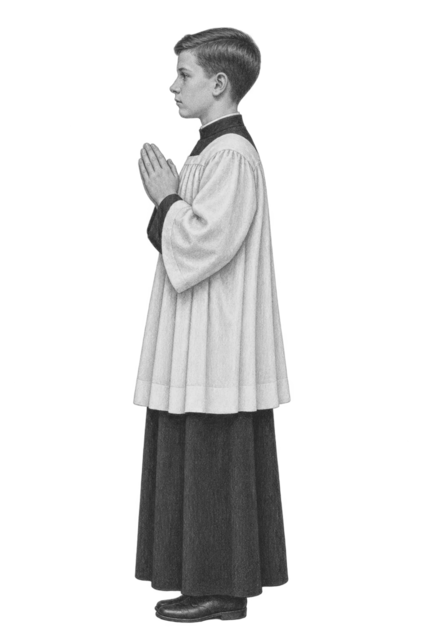
\includegraphics[height=23\ASGSceneUnit]{liturgy/roman-rite/1962/reference/altar-server-guides/shared/artwork/pencil/ASG-ART-037-server-facing-left.png}}};
  \ASGStation{#1}{#2-2}{#3}}
\newcommand{\LMMoveBookRight}[3]{%
  \node[anchor=south,inner sep=0pt] at (#1,#2) {\reflectbox{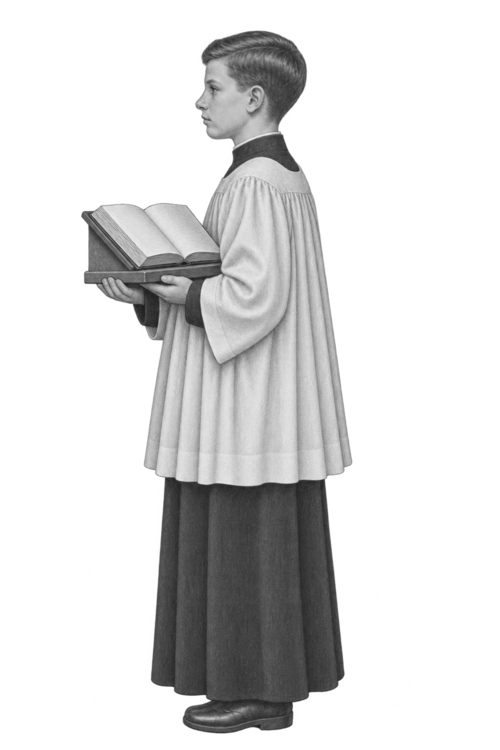
\includegraphics[height=23\ASGSceneUnit,trim=0 13 0 28,clip]{liturgy/roman-rite/1962/reference/altar-server-guides/shared/artwork/pencil/ASG-ART-040-server-carrying-missal.png}}};
  \ASGStation{#1}{#2-2}{#3}}
\newcommand{\LMMoveInstruction}[1]{%
  \par\smallskip{\fontsize{12}{14.5}\selectfont\RaggedRight #1\par}\smallskip}

\newcommand{\LMMoveBookRear}[3]{%
  \node[anchor=south,inner sep=0pt] at (#1,#2) {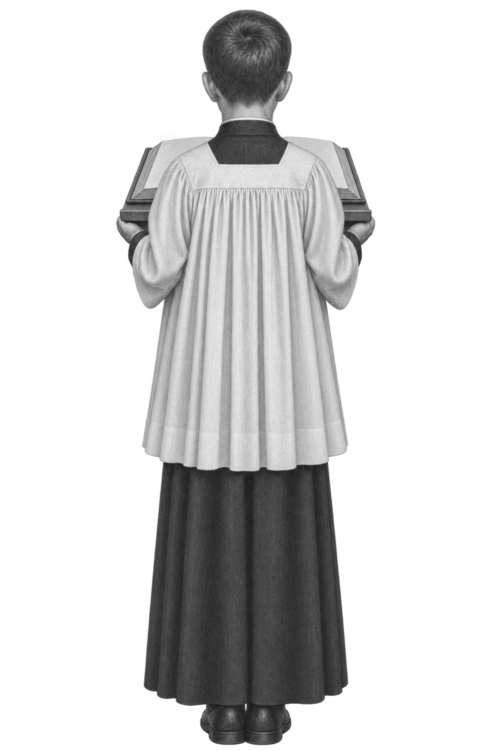
\includegraphics[height=23\ASGSceneUnit]{liturgy/roman-rite/1962/reference/altar-server-guides/shared/artwork/pencil/ASG-ART-053-server-carrying-missal-rear-v1.png}};
  \ASGStation{#1}{#2-2}{#3}}

\newcommand{\LMMoveMissalLift}{%
  \LMPositionScene{%
    \LMRestingCommunionPlate{91}{19.2}
    \LMRestingLavaboTowel{93.6}{19.6}\LMRestingLavaboBasin{93.6}{19.2}
    \LMCoveredChaliceObject{50}{43}
    \LMRestingCruets{97.2}{19.6}
    \ASGPriest{50}{26.5}{PRIEST}
    \ASGStandingServer{20}{11.3}{SECOND\\STAYS}
    \LMMoveBookRight{72}{26.5}{FIRST}
    \draw[asg route] (77,25) -- (81,23);
  }{1. First has lifted the Missal and stand together and turned toward the Epistle descent.}}
\newcommand{\LMMoveMissalDescent}{%
  \LMPositionScene{%
    \LMRestingCommunionPlate{91}{19.2}
    \LMRestingLavaboTowel{93.6}{19.6}\LMRestingLavaboBasin{93.6}{19.2}
    \LMCoveredChaliceObject{50}{43}
    \LMRestingCruets{97.2}{19.6}
    \ASGPriest{50}{26.5}{PRIEST}
    \ASGStandingServer{20}{11.3}{SECOND\\STAYS}
    \LMMoveBookRight{80}{18.3}{FIRST}
    \draw[asg route] (84,18) -- (86,12);
  }{2. First reaches the lowest step with both hands still supporting the book and stand.}}
\newcommand{\LMMoveMissalCentre}{%
  \LMPositionScene{%
    \LMRestingCommunionPlate{91}{19.2}
    \LMRestingLavaboTowel{93.6}{19.6}\LMRestingLavaboBasin{93.6}{19.2}
    \LMCoveredChaliceObject{50}{43}
    \LMRestingCruets{97.2}{19.6}
    \LMPriestAbove{50}{26.5}
    \ASGStandingServer{20}{11.3}{SECOND\\STAYS}
    \LMMoveBookRear{50}{11.3}{FIRST}
  }{3. At the centre, First stops and faces the altar with the book held securely.}}
\newcommand{\LMMoveMissalAscent}{%
  \LMPositionScene{%
    \LMRestingCommunionPlate{91}{19.2}
    \LMRestingLavaboTowel{93.6}{19.6}\LMRestingLavaboBasin{93.6}{19.2}
    \LMCoveredChaliceObject{50}{43}
    \LMRestingCruets{97.2}{19.6}
    \ASGPriest{50}{26.5}{PRIEST}
    \ASGStandingServer{20}{11.3}{SECOND\\STAYS}
    \LMMoveBookRear{31}{18.3}{FIRST}
    \draw[asg route] (36,19) -- (36,24);
  }{4. After the centre reverence, First turns up the Gospel steps with the book.}}
\newcommand{\LMMoveMissalPlaced}{%
  \LMPositionScene{%
    \LMRestingCommunionPlate{91}{19.2}
    \LMRestingLavaboTowel{93.6}{19.6}\LMRestingLavaboBasin{93.6}{19.2}
    \LMCoveredChaliceObject{50}{43}
    \LMRestingCruets{97.2}{19.6}
    \LMMissalAtGospel\ASGPriest{50}{26.5}{PRIEST}
    \ASGStandingServer{20}{11.3}{SECOND\\STAYS}
    \ASGStandingServer{31}{26.5}{FIRST}
  }{5. The book now rests at Gospel, angled toward the priest; First's hands are free.}}
\newcommand{\LMMoveMissalStepDown}{%
  \LMPositionScene{%
    \LMRestingCommunionPlate{91}{19.2}
    \LMRestingLavaboTowel{93.6}{19.6}\LMRestingLavaboBasin{93.6}{19.2}
    \LMCoveredChaliceObject{50}{43}
    \LMRestingCruets{97.2}{19.6}
    \LMMissalAtGospel\LMPriestFacingLeft{39}{26.5}{PRIEST}
    \ASGStandingServer{20}{11.3}{SECOND\\STAYS}
    \ASGStandingServer{29}{22.5}{FIRST}
  }{6. First has stepped down to Step 2 beside the book. Second has not moved up.}}
\newcommand{\LMMoveGospelDescent}{%
  \LMPositionScene{%
    \LMRestingCommunionPlate{91}{19.2}
    \LMRestingLavaboTowel{93.6}{19.6}\LMRestingLavaboBasin{93.6}{19.2}
    \LMCoveredChaliceObject{50}{43}
    \LMRestingCruets{97.2}{19.6}
    \LMMissalAtGospel\LMPriestFacingLeft{39}{26.5}{PRIEST}
    \ASGStandingServer{20}{11.3}{SECOND\\STAYS}
    \ASGServerFacingLeft{31}{18.3}{FIRST}
    \draw[asg route] (28,17) -- (28,12);
  }{1. Once the reading has begun, First steps down Gospel; the book stays on the altar.}}
\newcommand{\LMMoveGospelCentre}{%
  \LMPositionScene{%
    \LMRestingCommunionPlate{91}{19.2}
    \LMRestingLavaboTowel{93.6}{19.6}\LMRestingLavaboBasin{93.6}{19.2}
    \LMCoveredChaliceObject{50}{43}
    \LMRestingCruets{97.2}{19.6}
    \LMMissalAtGospel\LMPriestFacingLeft{39}{26.5}{PRIEST}
    \ASGStandingServer{20}{11.3}{SECOND\\STAYS}
    \ASGStandingServer{50}{11.3}{FIRST}
  }{2. First stops below the centre, faces the altar, and makes the taught reverence.}}
\newcommand{\LMMoveGospelCross}{%
  \LMPositionScene{%
    \LMRestingCommunionPlate{91}{19.2}
    \LMRestingLavaboTowel{93.6}{19.6}\LMRestingLavaboBasin{93.6}{19.2}
    \LMCoveredChaliceObject{50}{43}
    \LMRestingCruets{97.2}{19.6}
    \LMMissalAtGospel\LMPriestFacingLeft{39}{26.5}{PRIEST}
    \ASGStandingServer{20}{11.3}{SECOND\\STAYS}
    \LMMoveEmptyRight{62}{11.3}{FIRST}
    \draw[asg route] (66,7) -- (74,7);
  }{3. First walks along the floor toward Epistle, clear of the steps.}}
\newcommand{\LMMoveGospelReturned}{%
  \LMPositionScene{%
    \LMRestingCommunionPlate{91}{19.2}
    \LMRestingLavaboTowel{93.6}{19.6}\LMRestingLavaboBasin{93.6}{19.2}
    \LMCoveredChaliceObject{50}{43}
    \LMRestingCruets{97.2}{19.6}
    \LMMissalAtGospel\LMPriestFacingLeft{39}{26.5}{PRIEST}
    \ASGStandingServer{20}{11.3}{SECOND\\STAYS}
    \ASGServerFacingLeft{75}{11.3}{FIRST}
  }{4. At the normal Epistle place, First turns toward the Gospel. Both remain below the steps.}}

% Offertory: the named veil point is this guide's rehearsed Epistle pickup
% point, not a claim that every sanctuary uses this spot.
\newcommand{\LMMoveVeilSetDown}{%
  \LMPositionScene{%
    \LMUncoveredChaliceObject{60}{43}
    \LMRestingCommunionPlate{91}{19.2}
    \LMRestingLavaboTowel{93.6}{19.6}\LMRestingLavaboBasin{93.6}{19.2}
    \LMRestingCruets{97.2}{19.6}
    \LMMissalAtGospel\ASGPriest{50}{26.5}{PRIEST}
    \LMRestingVeil{70}{43}
    \ASGStandingServer{73}{26.5}{FIRST}
    \ASGStandingServer{25}{11.3}{SECOND\\WAITS}
    \ASGStation{82}{58}{VEIL PICKUP\\POINT}
  }{1. First has set the folded veil at the marked Epistle point; his hands are free.}}
\newcommand{\LMMoveVeilDescent}{%
  \LMPositionScene{%
    \LMUncoveredChaliceObject{60}{43}
    \LMRestingCommunionPlate{91}{19.2}
    \LMRestingLavaboTowel{93.6}{19.6}\LMRestingLavaboBasin{93.6}{19.2}
    \LMRestingCruets{97.2}{19.6}
    \LMMissalAtGospel\ASGPriest{50}{26.5}{PRIEST}
    \LMRestingVeil{70}{43}
    \LMMoveEmptyRight{80}{18.3}{FIRST}
    \ASGStandingServer{25}{11.3}{SECOND\\WAITS}
    \draw[asg route] (84,17) -- (84,12);
  }{2. First descends empty-handed. The folded veil stays at the same Epistle point.}}
\newcommand{\LMMoveOffertoryCentre}{%
  \LMPositionScene{%
    \LMUncoveredChaliceObject{60}{43}
    \LMRestingCommunionPlate{91}{19.2}
    \LMRestingLavaboTowel{93.6}{19.6}\LMRestingLavaboBasin{93.6}{19.2}
    \LMRestingCruets{97.2}{19.6}
    \LMMissalAtGospel\LMPriestAbove{50}{26.5}
    \LMRestingVeil{70}{43}
    \ASGStandingServer{57}{11.3}{FIRST}
    \ASGStandingServer{43}{11.3}{SECOND}
  }{3. Both meet on the floor at the centre, facing the altar with empty hands.}}
\newcommand{\LMMoveCredenceArrival}{%
  \LMPositionScene{%
    \LMUncoveredChaliceObject{60}{43}
    \LMRestingCommunionPlate{91}{19.2}
    \LMRestingLavaboTowel{93.6}{19.6}\LMRestingLavaboBasin{93.6}{19.2}
    \LMMissalAtGospel\ASGPriest{50}{26.5}{PRIEST}
    \LMRestingVeil{70}{43}\LMRestingCruets{97.2}{19.6}
    \LMMoveEmptyRight{83}{11.3}{FIRST}
    \LMMoveEmptyRight{70}{11.3}{SECOND}
    \draw[asg route] (76,6) -- (86,6);
  }{4. After the centre reverence, both reach the credence. The cruets are still on it.}}
\newcommand{\LMMoveCruetsTaken}{%
  \LMPositionScene{%
    \LMUncoveredChaliceObject{60}{43}
    \LMRestingCommunionPlate{91}{19.2}
    \LMRestingLavaboTowel{93.6}{19.6}\LMRestingLavaboBasin{93.6}{19.2}
    \LMMissalAtGospel\ASGPriest{50}{26.5}{PRIEST}
    \LMRestingVeil{70}{43}
    \LMWaitingCruetServer{75}{11.3}{FIRST}{2}
    \LMWaitingCruetServer{86}{11.3}{SECOND}{5}
    \ASGStation{74}{3}{FIRST: WINE\quad SECOND: WATER}
  }{5. First has taken wine and Second water. Both open cruets stay upright.}}
\newcommand{\LMMoveCruetsAscent}{%
  \LMPositionScene{%
    \LMUncoveredChaliceObject{60}{43}
    \LMRestingCommunionPlate{91}{19.2}
    \LMRestingLavaboTowel{93.6}{19.6}\LMRestingLavaboBasin{93.6}{19.2}
    \LMMissalAtGospel\ASGPriestFacingRight{66}{26.5}{PRIEST}
    \LMRestingVeil{70}{43}
    \LMWaitingCruetServer{75}{18.3}{FIRST}{2}
    \LMWaitingCruetServer{84}{18.3}{SECOND}{5}
    \draw[asg route] (70,19) -- (70,22);
  }{6. At the first step, both still hold their own cruets; continue to the Step 2 service place.}}
\newcommand{\LMMoveCruetsReset}{%
  \LMPositionScene{%
    \LMChaliceWithPallObject{50}{43}
    \LMRestingCommunionPlate{91}{19.2}
    \LMRestingLavaboTowel{93.6}{19.6}\LMRestingLavaboBasin{93.6}{19.2}
    \LMMissalAtGospel\ASGPriest{50}{26.5}{PRIEST}
    \LMRestingVeil{70}{43}\LMRestingCruets{97.2}{19.6}
    \LMMoveEmptyRight{83}{11.3}{FIRST}
    \LMMoveEmptyRight{71}{11.3}{SECOND}
  }{1. Back at the credence, both cruets are set down before the Lavabo equipment is taken.}}
\newcommand{\LMMoveLavaboEquipped}{%
  \LMPositionScene{%
    \LMChaliceWithPallObject{50}{43}
    \LMRestingCommunionPlate{91}{19.2}
    \LMRestingWineCruet{97.2}{19.6}
    \LMMissalAtGospel\ASGPriest{50}{26.5}{PRIEST}
    \LMRestingVeil{70}{43}
    \LMMoveTowelRear{85}{11.3}{FIRST}
    \LMMoveBowlRear{73}{11.3}{SECOND}
  }{2. First now holds the open towel; Second holds the bowl and upright water cruet.}}
\newcommand{\LMMoveLavaboAscent}{%
  \LMPositionScene{%
    \LMChaliceWithPallObject{50}{43}
    \LMRestingCommunionPlate{91}{19.2}
    \LMRestingWineCruet{97.2}{19.6}
    \LMMissalAtGospel\ASGPriestFacingRight{61}{26.5}{PRIEST}
    \LMRestingVeil{70}{43}
    \LMMoveTowelRear{81}{18.3}{FIRST}
    \LMMoveBowlRear{70}{18.3}{SECOND}
    \draw[asg route] (67,19) -- (67,22);
  }{3. Carry the changed equipment up Epistle: Second keeps bowl and water level, First keeps the towel clear.}}
\newcommand{\LMMoveBellTaken}{%
  \LMPositionScene{%
    \LMChaliceWithPallObject{50}{43}
    \LMRestingCommunionPlate{91}{19.2}
    \LMRestingLavaboTowel{93.6}{19.6}\LMRestingLavaboBasin{93.6}{19.2}
    \LMMissalAtGospel\ASGPriest{50}{26.5}{PRIEST}
    \LMRestingVeil{70}{43}\LMRestingCruets{97.2}{19.6}
    \LMMoveBellRear{80}{11.3}{FIRST}
    \ASGStandingServer{68}{11.3}{SECOND}
  }{1. Lavabo articles are reset. First now holds the bell; Second's hands are free.}}
\newcommand{\LMMoveBellCentre}{%
  \LMPositionScene{%
    \LMChaliceWithPallObject{50}{43}
    \LMRestingCommunionPlate{91}{19.2}
    \LMRestingLavaboTowel{93.6}{19.6}\LMRestingLavaboBasin{93.6}{19.2}
    \LMRestingCruets{97.2}{19.6}
    \LMMissalAtGospel\LMPriestAbove{50}{26.5}
    \LMRestingVeil{70}{43}
    \LMMoveBellAtAltar{57}{11.3}{FIRST}
    \ASGStandingServer{43}{11.3}{SECOND}
  }{2. Both stop facing the altar at the centre. First keeps the bell still during the reverence.}}
\newcommand{\LMMoveBellAtNormalPlace}{%
  \LMPositionScene{%
    \LMChaliceWithPallObject{50}{43}
    \LMRestingCommunionPlate{91}{19.2}
    \LMRestingLavaboTowel{93.6}{19.6}\LMRestingLavaboBasin{93.6}{19.2}
    \LMRestingCruets{97.2}{19.6}
    \LMMissalAtGospel\ASGPriest{50}{26.5}{PRIEST}
    \LMRestingVeil{70}{43}
    \LMMoveBellAtAltar{75}{11.3}{FIRST}
    \ASGStandingServer{25}{11.3}{SECOND}
  }{3. Both have returned to their normal floor places. First still holds the bell before setting it down.}}

\newcommand{\LMMoveCruetsRear}[3]{%
  \node[anchor=south,inner sep=0pt] at (#1,#2) {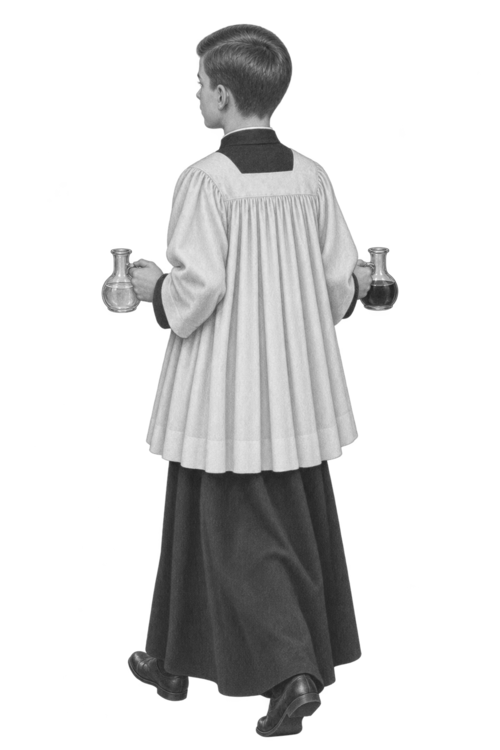
\includegraphics[height=23\ASGSceneUnit]{liturgy/roman-rite/1962/reference/altar-server-guides/shared/artwork/pencil/ASG-ART-054-server-carrying-two-cruets-v1.png}};
  \ASGStation{#1}{#2-2}{#3}}

\newcommand{\LMMoveBellRear}[3]{%
  \node[anchor=south,inner sep=0pt] at (#1,#2) {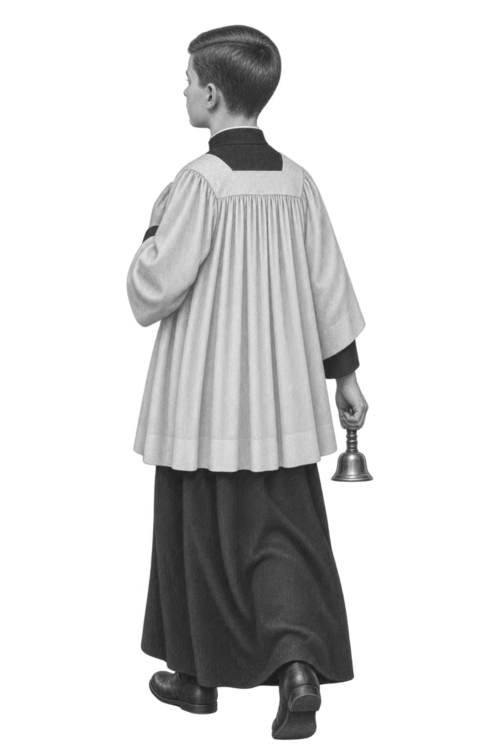
\includegraphics[height=23\ASGSceneUnit]{liturgy/roman-rite/1962/reference/altar-server-guides/shared/artwork/pencil/ASG-ART-055-server-carrying-bell-right-v1.png}};
  \ASGStation{#1}{#2-2}{#3}}

\newcommand{\LMMoveBowlRear}[3]{%
  \node[anchor=south,inner sep=0pt] at (#1,#2) {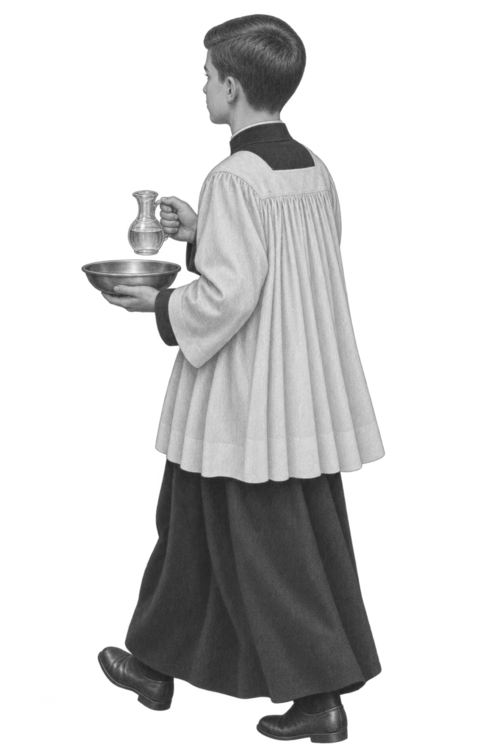
\includegraphics[height=23\ASGSceneUnit]{liturgy/roman-rite/1962/reference/altar-server-guides/shared/artwork/pencil/ASG-ART-056-server-carrying-bowl-water-v1.png}};
  \ASGStation{#1}{#2-2}{#3}}

\newcommand{\LMMoveTowelRear}[3]{%
  \node[anchor=south,inner sep=0pt] at (#1,#2) {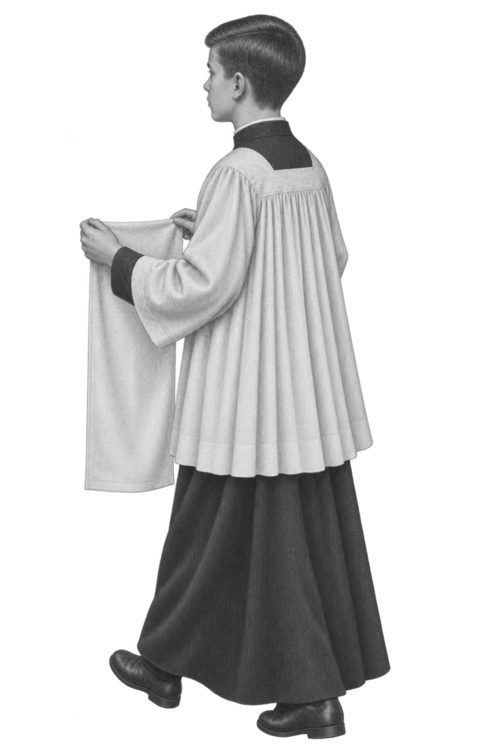
\includegraphics[height=23\ASGSceneUnit]{liturgy/roman-rite/1962/reference/altar-server-guides/shared/artwork/pencil/ASG-ART-057-server-carrying-open-towel-v1.png}};
  \ASGStation{#1}{#2-2}{#3}}

\newcommand{\LMMoveLavaboReady}{%
  \LMPositionScene{%
    \LMChaliceWithPallObject{50}{43}
    \LMRestingCommunionPlate{91}{19.2}
    \LMRestingWineCruet{97.2}{19.6}
    \LMMissalAtGospel\ASGPriestFacingRight{61}{26.5}{PRIEST}
    \LMRestingVeil{70}{43}
    \LMMoveTowelRear{81}{22.5}{FIRST}
    \LMMoveBowlRear{70}{22.5}{SECOND}
  }{4. Both arrive at Step 2 with the same equipment. Stop, bow together, and face the priest before washing.}}

\newcommand{\LMMoveElevationFirstStep}{%
  \LMPositionScene{%
    \LMChaliceWithPallObject{50}{43}
    \LMRestingCommunionPlate{91}{19.2}
    \LMRestingLavaboTowel{93.6}{19.6}\LMRestingLavaboBasin{93.6}{19.2}
    \LMRestingCruets{97.2}{19.6}
    \LMMissalAtGospel\ASGPriest{50}{26.5}{PRIEST}
    \LMRestingVeil{70}{43}
    \LMMoveBellRear{74}{18.3}{FIRST}
    \ASGStandingServer{26}{18.3}{SECOND}
    \draw[asg route] (69,19) -- (64,22);
    \draw[asg route] (31,19) -- (36,22);
  }{1. After the warning, both have risen and begun the short ascent. First carries the bell in his right hand.}}

\newcommand{\LMMoveElevationSecondStep}{%
  \LMPositionScene{%
    \LMChaliceWithPallObject{50}{43}
    \LMRestingCommunionPlate{91}{19.2}
    \LMRestingLavaboTowel{93.6}{19.6}\LMRestingLavaboBasin{93.6}{19.2}
    \LMRestingCruets{97.2}{19.6}
    \LMMissalAtGospel\ASGPriest{50}{26.5}{PRIEST}
    \LMRestingVeil{70}{43}
    \LMMoveBellRear{62}{22.5}{FIRST}
    \ASGStandingServer{38}{22.5}{SECOND}
  }{2. Both reach Step 2 on their own sides; next ascend to the predella and kneel slightly behind the priest.}}

\newcommand{\LMMoveElevationDescent}{%
  \LMPositionScene{%
    \LMChaliceWithPallObject{50}{43}
    \LMRestingCommunionPlate{91}{19.2}
    \LMRestingLavaboTowel{93.6}{19.6}\LMRestingLavaboBasin{93.6}{19.2}
    \LMRestingCruets{97.2}{19.6}
    \LMMissalAtGospel\ASGPriest{50}{26.5}{PRIEST}
    \LMRestingVeil{70}{43}
    \LMMoveBellFront{64}{18.3}{FIRST}
    \LMMoveEmptyRight{36}{18.3}{SECOND}
    \draw[asg route] (63,17) -- (60,12);
    \draw[asg route] (35,17) -- (40,12);
  }{1. After the final reverence, both descend. First keeps the bell upright and silent.}}

\newcommand{\LMMoveElevationCentre}{%
  \LMPositionScene{%
    \LMChaliceWithPallObject{50}{43}
    \LMRestingCommunionPlate{91}{19.2}
    \LMRestingLavaboTowel{93.6}{19.6}\LMRestingLavaboBasin{93.6}{19.2}
    \LMRestingCruets{97.2}{19.6}
    \LMMissalAtGospel\LMPriestAbove{50}{26.5}
    \LMRestingVeil{70}{43}
    \LMMoveBellAtAltar{57}{11.3}{FIRST}
    \ASGStandingServer{43}{11.3}{SECOND}
  }{2. Both stop on the floor facing the altar. First still has the bell for the centre reverence.}}

\newcommand{\LMMoveAblutionTaken}{%
  \LMPositionScene{%
    \LMRestingCommunionPlate{60}{43}
    \LMUncoveredChaliceObject{50}{43}
    \LMRestingLavaboTowel{93.6}{19.6}\LMRestingLavaboBasin{93.6}{19.2}
    \LMRestingBell{80}{22.5}
    \LMMissalAtGospel\ASGPriest{50}{26.5}{PRIEST}
    \LMRestingVeil{70}{43}
    \ASGStandingServer{25}{11.3}{SECOND\\WAITS}
    \LMMoveCruetsRear{83}{11.3}{FIRST}
  }{1. First leaves the credence with wine in his right hand and water in his left. Second is standing below Gospel.}}

\newcommand{\LMMoveAblutionAscent}{%
  \LMPositionScene{%
    \LMRestingCommunionPlate{60}{43}
    \LMUncoveredChaliceObject{50}{43}
    \LMRestingLavaboTowel{93.6}{19.6}\LMRestingLavaboBasin{93.6}{19.2}
    \LMRestingBell{80}{22.5}
    \LMMissalAtGospel\ASGPriest{50}{26.5}{PRIEST}
    \LMRestingVeil{70}{43}
    \ASGStandingServer{25}{11.3}{SECOND\\WAITS}
    \LMMoveCruetsRear{78}{18.3}{FIRST}
    \draw[asg route] (73,19) -- (73,22);
  }{2. First carries both upright cruets up Epistle toward Step 2; Second leaves the lane clear.}}

\newcommand{\LMMoveAblutionStepTwo}{%
  \LMPositionScene{%
    \LMRestingCommunionPlate{60}{43}
    \LMUncoveredChaliceObject{50}{43}
    \LMRestingLavaboTowel{93.6}{19.6}\LMRestingLavaboBasin{93.6}{19.2}
    \LMRestingBell{80}{22.5}
    \LMMissalAtGospel\ASGPriest{50}{26.5}{PRIEST}
    \LMRestingVeil{70}{43}
    \ASGStandingServer{25}{11.3}{SECOND\\WAITS}
    \LMMoveCruetsRear{76}{22.5}{FIRST}
  }{3. First reaches the waiting step at Epistle. Stop here until the priest offers the chalice.}}

\newcommand{\LMMoveAblutionPredella}{%
  \LMPositionScene{%
    \LMRestingCommunionPlate{60}{43}
    \LMRestingLavaboTowel{93.6}{19.6}\LMRestingLavaboBasin{93.6}{19.2}
    \LMRestingBell{80}{22.5}
    \LMMissalAtGospel\LMMovePriestWithChalice{50}{26.5}{PRIEST}
    \LMRestingVeil{70}{43}
    \ASGStandingServer{25}{11.3}{SECOND\\WAITS}
    \LMMoveCruetsRear{68}{26.5}{FIRST}
    \draw[asg route] (63,25) -- (59,25);
  }{4. At the priest's cue, First has ascended to the predella and approaches the centre with both cruets.}}

\newcommand{\LMMoveAblutionDown}{%
  \LMPositionScene{%
    \LMRestingCommunionPlate{60}{43}
    \LMRestingLavaboTowel{93.6}{19.6}\LMRestingLavaboBasin{93.6}{19.2}
    \LMRestingBell{80}{22.5}
    \LMMissalAtGospel\LMMovePriestWithChalice{50}{26.5}{PRIEST}
    \LMRestingVeil{70}{43}
    \ASGStandingServer{25}{11.3}{SECOND\\WAITS}
    \LMMoveCruetsFront{76}{22.5}{FIRST}
  }{After the first wine pour, First steps back down to Step 2 carrying both cruets; wait for the priest to come to Epistle.}}

\newcommand{\LMMoveAblutionReturn}{%
  \LMPositionScene{%
    \LMRestingCommunionPlate{60}{43}
    \LMUncoveredChaliceObject{44}{43}
    \LMRestingLavaboTowel{93.6}{19.6}\LMRestingLavaboBasin{93.6}{19.2}
    \LMRestingBell{80}{22.5}
    \LMMissalAtGospel\ASGPriest{63}{26.5}{PRIEST}
    \LMRestingVeil{70}{43}
    \ASGStandingServer{25}{11.3}{SECOND\\WAITS}
    \LMMoveCruetsFront{81}{18.3}{FIRST}
    \draw[asg route] (85,17) -- (88,12);
  }{1. After the water pour and the priest's signal, First descends with both cruets to return them to the credence.}}

\newcommand{\LMMoveAblutionReset}{%
  \LMPositionScene{%
    \LMRestingCommunionPlate{60}{43}
    \LMUncoveredChaliceObject{44}{43}
    \LMRestingLavaboTowel{93.6}{19.6}\LMRestingLavaboBasin{93.6}{19.2}
    \LMRestingBell{80}{22.5}
    \LMMissalAtGospel\ASGPriest{50}{26.5}{PRIEST}
    \LMRestingVeil{70}{43}
    \ASGStandingServer{25}{11.3}{SECOND\\WAITS}
    \LMRestingCruets{97.2}{19.6}
    \LMMoveEmptyRight{83}{11.3}{FIRST}
  }{2. Both cruets are back on the credence. First is empty-handed before any cleared Communion plate is retrieved.}}

\newcommand{\LMMoveExchangeTaken}{%
  \LMPositionScene{%
    \LMUncoveredChaliceObject{44}{43}
    \LMRestingCommunionPlate{91}{19.2}
    \LMRestingLavaboTowel{93.6}{19.6}\LMRestingLavaboBasin{93.6}{19.2}
    \LMRestingCruets{97.2}{19.6}\LMRestingBell{80}{22.5}
    \ASGPriest{50}{26.5}{PRIEST}
    \LMBookBearer{29}{18.3}{SECOND}
    \LMMoveVeilRight{78}{18.3}{FIRST}
  }{1. Second descends Gospel with the Missal and stand; First descends Epistle with the folded veil.}}

\newcommand{\LMMoveExchangeYield}{%
  \LMPositionScene{%
    \LMUncoveredChaliceObject{44}{43}
    \LMRestingCommunionPlate{91}{19.2}
    \LMRestingLavaboTowel{93.6}{19.6}\LMRestingLavaboBasin{93.6}{19.2}
    \LMRestingCruets{97.2}{19.6}\LMRestingBell{80}{22.5}
    \LMPriestAbove{50}{26.5}
    \LMMoveBookRight{55}{11.3}{SECOND}
    \LMVeilBearer{76}{11.3}{FIRST}
    \ASGStop{68}{8}{A}
    \draw[asg route] (60,8) -- (66,8);
    \ASGStation{79}{51}{FIRST WAITS\\BEFORE A}
  }{2. At the marked floor crossing A, First waits with the veil while Second passes toward Epistle with the book.}}

\newcommand{\LMMoveExchangeClear}{%
  \LMPositionScene{%
    \LMUncoveredChaliceObject{44}{43}
    \LMRestingCommunionPlate{91}{19.2}
    \LMRestingLavaboTowel{93.6}{19.6}\LMRestingLavaboBasin{93.6}{19.2}
    \LMRestingCruets{97.2}{19.6}\LMRestingBell{80}{22.5}
    \LMPriestAbove{50}{26.5}
    \LMMoveBookRear{76}{18.3}{SECOND}
    \LMVeilBearer{58}{11.3}{FIRST}
    \ASGStop{68}{8}{A}
    \draw[asg route] (52,7) -- (44,7);
  }{3. Second has cleared A and is going up Epistle. First can now cross below the steps toward Gospel.}}

\newcommand{\LMMoveExchangeBookPlaced}{%
  \LMPositionScene{%
    \LMUncoveredChaliceObject{44}{43}
    \LMRestingCommunionPlate{91}{19.2}
    \LMRestingLavaboTowel{93.6}{19.6}\LMRestingLavaboBasin{93.6}{19.2}
    \LMRestingCruets{97.2}{19.6}\LMRestingBell{80}{22.5}
    \ASGPriest{50}{26.5}{PRIEST}
    \LMMissalAtEpistle
    \ASGStandingServer{73}{26.5}{SECOND}
    \LMVeilBearer{29}{18.3}{FIRST}
    \draw[asg route] (25,19) -- (25,24);
  }{4. The Missal and stand now rest straight at Epistle. First reaches the Gospel steps with the veil.}}

\newcommand{\LMMoveExchangeVeilPlaced}{%
  \LMPositionScene{%
    \LMUncoveredChaliceObject{44}{43}
    \LMRestingCommunionPlate{91}{19.2}
    \LMRestingLavaboTowel{93.6}{19.6}\LMRestingLavaboBasin{93.6}{19.2}
    \LMRestingCruets{97.2}{19.6}\LMRestingBell{80}{22.5}
    \ASGPriest{50}{26.5}{PRIEST}
    \LMMissalAtEpistle\LMRestingVeil{31}{43}
    \ASGStandingServer{29}{26.5}{FIRST}
    \ASGStandingServer{73}{26.5}{SECOND}
  }{5. The folded veil now rests at the Gospel point. Both have released their objects and have empty hands.}}

\newcommand{\LMMoveExchangeEmptyDescent}{%
  \LMPositionScene{%
    \LMUncoveredChaliceObject{44}{43}
    \LMRestingCommunionPlate{91}{19.2}
    \LMRestingLavaboTowel{93.6}{19.6}\LMRestingLavaboBasin{93.6}{19.2}
    \LMRestingCruets{97.2}{19.6}\LMRestingBell{80}{22.5}
    \ASGPriest{50}{26.5}{PRIEST}
    \LMMissalAtEpistle\LMRestingVeil{31}{43}
    \ASGServerFacingLeft{28}{18.3}{FIRST}
    \LMMoveEmptyRight{78}{18.3}{SECOND}
    \draw[asg route] (25,17) -- (25,12);
    \draw[asg route] (82,17) -- (82,12);
  }{6. Both descend empty-handed from the sides where they placed the objects.}}

\newcommand{\LMMoveExchangeCentre}{%
  \LMPositionScene{%
    \LMUncoveredChaliceObject{44}{43}
    \LMRestingCommunionPlate{91}{19.2}
    \LMRestingLavaboTowel{93.6}{19.6}\LMRestingLavaboBasin{93.6}{19.2}
    \LMRestingCruets{97.2}{19.6}\LMRestingBell{80}{22.5}
    \LMPriestAbove{50}{26.5}
    \LMMissalAtEpistle\LMRestingVeil{31}{43}
    \ASGStandingServer{43}{11.3}{FIRST}
    \ASGStandingServer{57}{11.3}{SECOND}
  }{7. Both stop facing the altar at the centre. Make the taught reverence before returning to the normal sides.}}

\newcommand{\LMMoveExchangeReturn}{%
  \LMPositionScene{%
    \LMUncoveredChaliceObject{44}{43}
    \LMRestingCommunionPlate{91}{19.2}
    \LMRestingLavaboTowel{93.6}{19.6}\LMRestingLavaboBasin{93.6}{19.2}
    \LMRestingCruets{97.2}{19.6}\LMRestingBell{80}{22.5}
    \ASGPriest{50}{26.5}{PRIEST}
    \LMMissalAtEpistle\LMRestingVeil{31}{43}
    \LMMoveEmptyRight{66}{11.3}{FIRST}
    \ASGServerFacingLeft{33}{11.3}{SECOND}
    \draw[asg route] (68,6) -- (75,6);
    \draw[asg route] (31,6) -- (25,6);
  }{8. Following the rehearsed passing order, First returns toward Epistle and Second toward Gospel, both empty-handed.}}

\newcommand{\LMMoveEndingServers}{%
  \LMPositionScene{%
    \LMRestingCommunionPlate{91}{19.2}
    \LMRestingLavaboTowel{93.6}{19.6}\LMRestingLavaboBasin{93.6}{19.2}
    \LMRestingCruets{97.2}{19.6}\LMRestingBell{80}{22.5}
    \LMMissalAtEpistle\LMCoveredChaliceObject{50}{43}\ASGPriest{50}{26.5}{PRIEST}
    \LMMoveEmptyRight{29}{11.3}{SECOND}
    \ASGServerFacingLeft{71}{11.3}{FIRST}
    \draw[asg route] (32,6) -- (40,6);
    \draw[asg route] (68,6) -- (60,6);
  }{1. After the Last Gospel, both move inward along the floor toward the foot; the priest remains at the altar.}}

\newcommand{\LMMoveEndingPriestDown}{%
  \LMPositionScene{%
    \LMRestingCommunionPlate{91}{19.2}
    \LMRestingLavaboTowel{93.6}{19.6}\LMRestingLavaboBasin{93.6}{19.2}
    \LMRestingCruets{97.2}{19.6}\LMRestingBell{80}{22.5}
    \LMMissalAtEpistle
    \LMMovePriestChaliceFront{50}{18.3}{PRIEST}
    \ASGStandingServer{33}{11.3}{SECOND}
    \ASGStandingServer{67}{11.3}{FIRST}
  }{2. The priest descends carrying the covered chalice. The servers wait at the foot with the centre clear.}}

\newcommand{\LMMoveEndingForm}{%
  \LMPositionScene{%
    \LMRestingCommunionPlate{91}{19.2}
    \LMRestingLavaboTowel{93.6}{19.6}\LMRestingLavaboBasin{93.6}{19.2}
    \LMRestingCruets{97.2}{19.6}\LMRestingBell{80}{22.5}
    \LMMissalAtEpistle
    \LMChaliceBearer{50}{11.3}{PRIEST}
    \ASGServerFacingLeft{20}{11.3}{FIRST}
    \ASGServerFacingLeft{35}{11.3}{SECOND}
  }{After the common floor reverence, both turn into the departure line: First leads, Second follows, then the priest.}}

\newcommand{\LMMoveBellFront}[3]{%
  \node[anchor=south,inner sep=0pt] at (#1,#2) {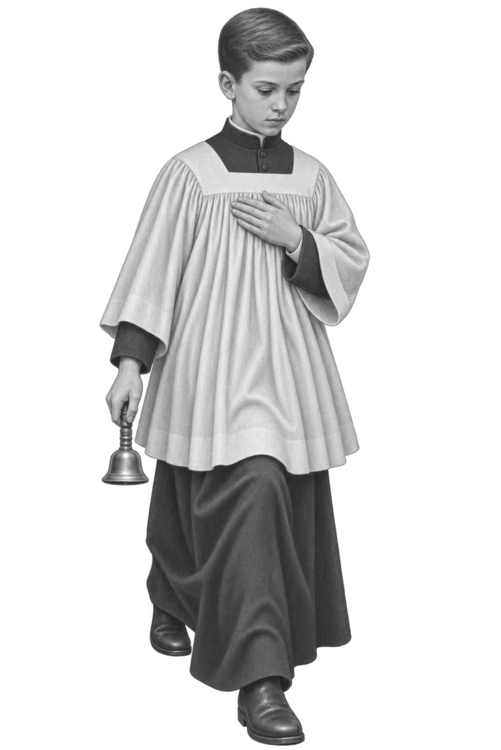
\includegraphics[height=23\ASGSceneUnit]{liturgy/roman-rite/1962/reference/altar-server-guides/shared/artwork/pencil/ASG-ART-064-server-descending-bell-right-v1.png}};
  \ASGStation{#1}{#2-2}{#3}}

\newcommand{\LMMoveCruetsFront}[3]{%
  \node[anchor=south,inner sep=0pt] at (#1,#2) {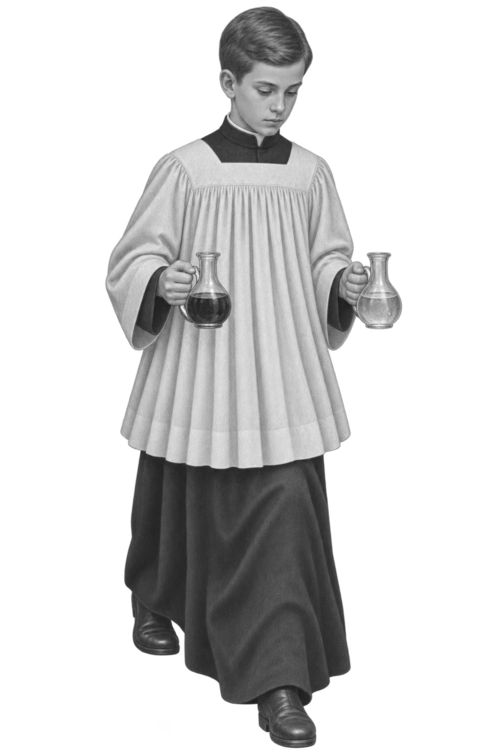
\includegraphics[height=23\ASGSceneUnit]{liturgy/roman-rite/1962/reference/altar-server-guides/shared/artwork/pencil/ASG-ART-065-server-descending-two-cruets-v1.png}};
  \ASGStation{#1}{#2-2}{#3}}

\newcommand{\LMMovePriestChaliceFront}[3]{%
  \node[anchor=south,inner sep=0pt] at (#1,#2) {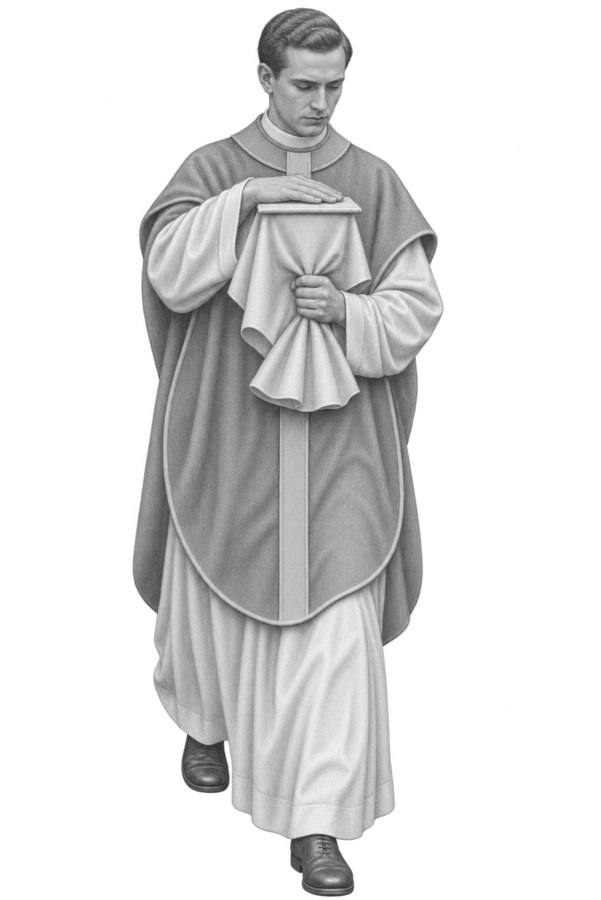
\includegraphics[height=28\ASGSceneUnit]{liturgy/roman-rite/1962/reference/altar-server-guides/shared/artwork/pencil/ASG-ART-066-priest-descending-covered-chalice-v1.png}};
  \ASGStation{#1}{#2-2}{#3}}

\newcommand{\LMMoveBellAtAltar}[3]{%
  \node[anchor=south,inner sep=0pt] at (#1,#2) {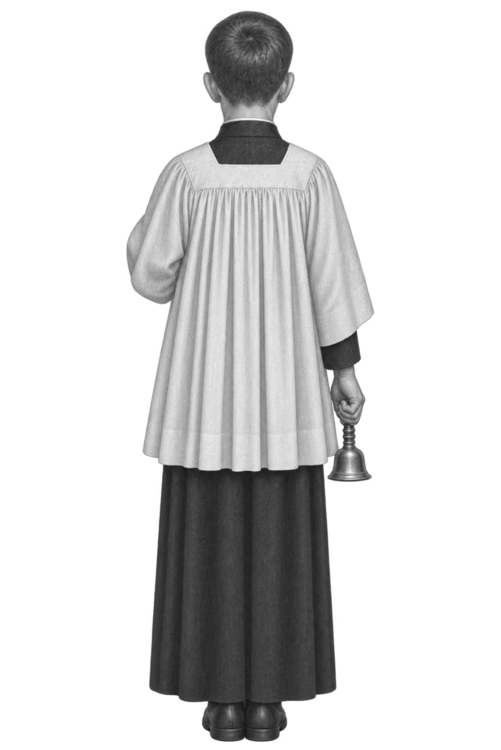
\includegraphics[height=23\ASGSceneUnit]{liturgy/roman-rite/1962/reference/altar-server-guides/shared/artwork/pencil/ASG-ART-067-server-standing-bell-right-rear-v1.png}};
  \ASGStation{#1}{#2-2}{#3}}

\newcommand{\LMMovePriestWithChalice}[3]{%
  \node[anchor=south,inner sep=0pt] at (#1,#2) {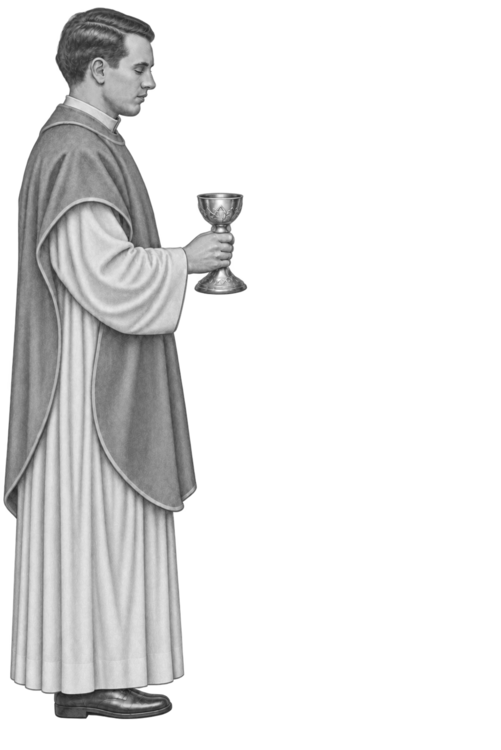
\includegraphics[height=28\ASGSceneUnit,trim=0 30 245 7,clip]{liturgy/roman-rite/1962/reference/altar-server-guides/shared/artwork/pencil/ASG-ART-075-priest-holding-uncovered-chalice.png}};
  \ASGStation{#1}{#2-2}{#3}}


% The rear priest is an orientation silhouette at this stopped moment. The
% covered chalice remains held in front and is honestly occluded by his body.
\newcommand{\LMMoveArrivalLine}{%
  \LMPositionScene{%
    \LMRestingCommunionPlate{91}{19.2}
    \LMRestingLavaboTowel{93.6}{19.6}\LMRestingLavaboBasin{93.6}{19.2}
    \LMRestingCruets{97.2}{19.6}
    \LMMissalAtEpistle
    \ASGServerFacingLeft{41}{11.3}{FIRST}
    \ASGServerFacingLeft{59}{11.3}{SECOND}
    \LMChaliceBearer{79}{11.3}{PRIEST}
    \draw[asg route] (35,6) -- (28,6);
  }{First leads, Second follows, and the priest carries the covered chalice behind them.}}
\newcommand{\LMMoveArrivalFacing}{%
  \LMPositionScene{%
    \LMRestingCommunionPlate{91}{19.2}
    \LMRestingLavaboTowel{93.6}{19.6}\LMRestingLavaboBasin{93.6}{19.2}
    \LMRestingCruets{97.2}{19.6}
    \LMMissalAtEpistle
    \ASGPriest{50}{11.3}{PRIEST}
    \ASGStandingServer{67}{11.3}{FIRST}
    \ASGStandingServer{33}{11.3}{SECOND}
  }{All have stopped facing the altar. The priest still holds the covered chalice in front, hidden by his back.}}
\newcommand{\LMMoveDepartureFacing}{%
  \LMPositionScene{%
    \LMRestingCommunionPlate{91}{19.2}
    \LMRestingLavaboTowel{93.6}{19.6}\LMRestingLavaboBasin{93.6}{19.2}
    \LMRestingCruets{97.2}{19.6}\LMRestingBell{80}{22.5}
    \LMMissalAtEpistle
    \ASGPriest{50}{11.3}{PRIEST}
    \ASGStandingServer{67}{11.3}{FIRST}
    \ASGStandingServer{33}{11.3}{SECOND}
  }{3. At the foot, all stop facing the altar. The priest's covered chalice remains held in front, hidden by his back.}}

\newcommand{\LMMoveVeilRight}[3]{%
  \node[anchor=south,inner sep=0pt] at (#1,#2) {\reflectbox{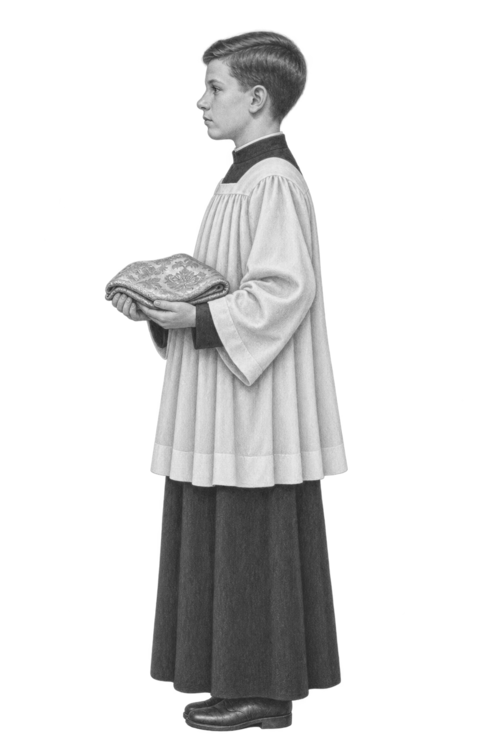
\includegraphics[height=23\ASGSceneUnit]{liturgy/roman-rite/1962/reference/altar-server-guides/shared/artwork/pencil/ASG-ART-052-server-carrying-folded-veil.png}}};
  \ASGStation{#1}{#2-2}{#3}}


% The plate carry is symmetric: both hands support the handle and underside.
% Its return view may be mirrored; no handed liturgical action is reversed.
\newcommand{\LMMovePlateLeft}[3]{%
  \node[anchor=south,inner sep=0pt] at (#1,#2) {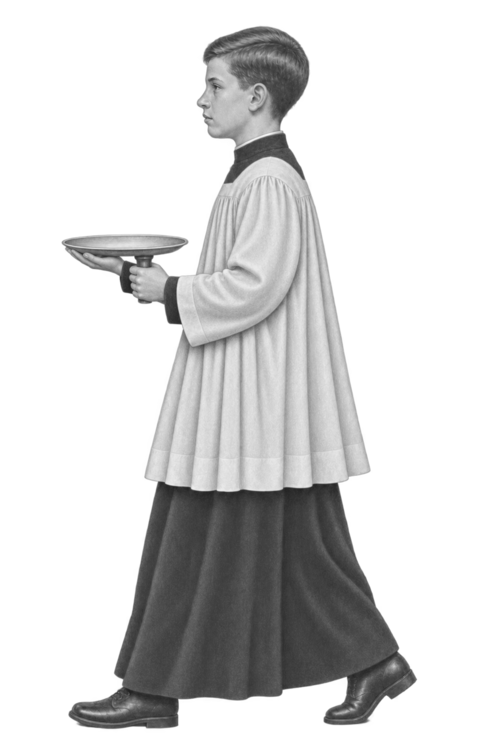
\includegraphics[height=23\ASGSceneUnit]{liturgy/roman-rite/1962/reference/altar-server-guides/shared/artwork/pencil/ASG-ART-077-server-carrying-communion-plate.png}};
  \ASGStation{#1}{#2-2}{#3}}
\newcommand{\LMMovePlateRight}[3]{%
  \node[anchor=south,inner sep=0pt] at (#1,#2) {\reflectbox{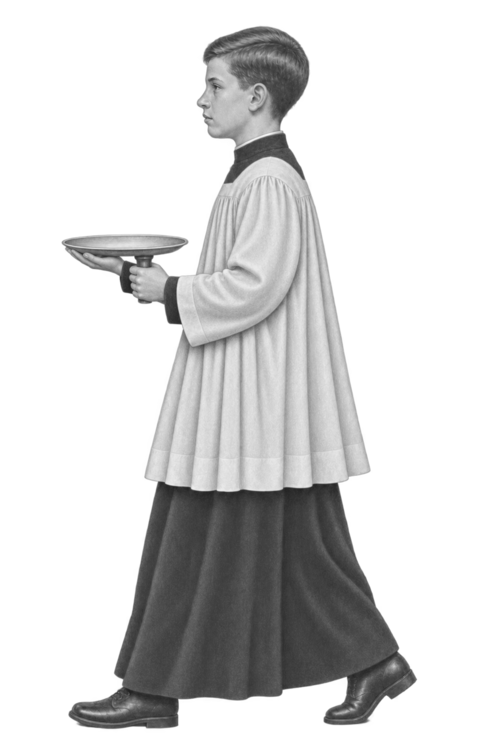
\includegraphics[height=23\ASGSceneUnit]{liturgy/roman-rite/1962/reference/altar-server-guides/shared/artwork/pencil/ASG-ART-077-server-carrying-communion-plate.png}}};
  \ASGStation{#1}{#2-2}{#3}}
\newcommand{\LMMovePlateTaken}{%
  \LMPositionScene{%
    \LMRestingLavaboTowel{93.6}{19.6}\LMRestingLavaboBasin{93.6}{19.2}
    \LMRestingCruets{97.2}{19.6}\LMRestingBell{80}{22.5}
    \LMChaliceWithPallObject{50}{43}\LMRestingVeil{70}{43}
    \LMMissalAtGospel\ASGPriest{50}{26.5}{PRIEST}
    \ASGKneelingServer{25}{18.3}{SECOND\\WAITS}
    \LMMovePlateLeft{79}{11.3}{FIRST}
    \draw[asg route] (73,6) -- (65,6);
  }{1. First leaves the credence carrying the Communion plate level in both hands; it is no longer on the table.}}
\newcommand{\LMMovePlateApproach}{%
  \LMPositionScene{%
    \LMRestingLavaboTowel{93.6}{19.6}\LMRestingLavaboBasin{93.6}{19.2}
    \LMRestingCruets{97.2}{19.6}\LMRestingBell{80}{22.5}
    \LMChaliceWithPallObject{50}{43}\LMRestingVeil{70}{43}
    \LMMissalAtGospel\LMPriestAbove{50}{26.5}
    \ASGKneelingServer{25}{18.3}{SECOND\\WAITS}
    \LMMovePlateLeft{48}{11.3}{FIRST}
  }{2. First reaches the rehearsed floor approach point, ready to join the priest's right when he comes to distribute.}}
\newcommand{\LMMovePlateCollected}{%
  \LMPositionScene{%
    \LMRestingLavaboTowel{93.6}{19.6}\LMRestingLavaboBasin{93.6}{19.2}
    \LMRestingCruets{97.2}{19.6}\LMRestingBell{80}{22.5}
    \LMUncoveredChaliceObject{44}{43}\LMRestingVeil{70}{43}
    \LMMissalAtGospel\ASGPriest{50}{26.5}{PRIEST}
    \ASGStandingServer{25}{11.3}{SECOND\\WAITS}
    \LMMovePlateRight{77}{26.5}{FIRST}
    \draw[asg route] (82,25) -- (85,21);
  }{1. After the final water and the priest's signal, First has collected the cleared plate at Epistle and turned to descend.}}
\newcommand{\LMMovePlateReturning}{%
  \LMPositionScene{%
    \LMRestingLavaboTowel{93.6}{19.6}\LMRestingLavaboBasin{93.6}{19.2}
    \LMRestingCruets{97.2}{19.6}\LMRestingBell{80}{22.5}
    \LMUncoveredChaliceObject{44}{43}\LMRestingVeil{70}{43}
    \LMMissalAtGospel\ASGPriest{50}{26.5}{PRIEST}
    \ASGStandingServer{25}{11.3}{SECOND\\WAITS}
    \LMMovePlateRight{83}{11.3}{FIRST}
    \draw[asg route] (85,6) -- (90,6);
  }{2. Back on the floor, First carries the cleared plate toward the credence; keep it level until it rests on the table.}}
